\documentclass{standalone}
\usepackage{tikz}
\usetikzlibrary{decorations.pathreplacing}
\begin{document}

            % TIKZ
            %$\left\{
                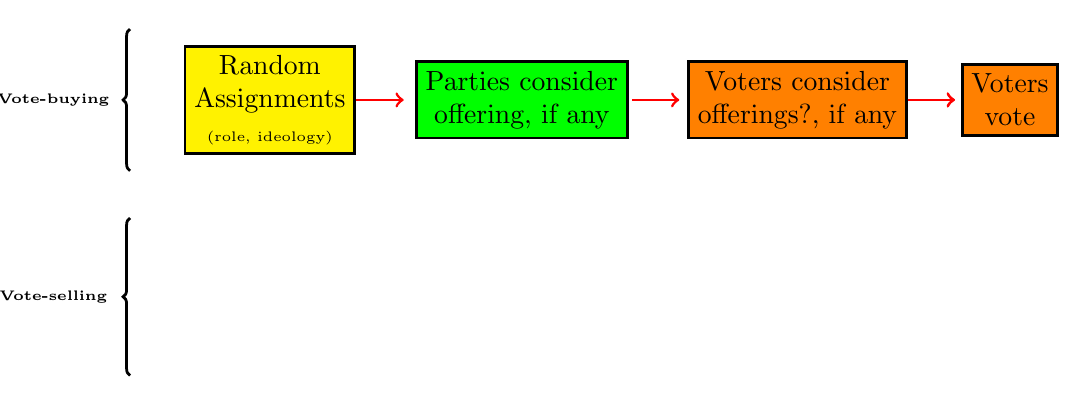
\begin{tikzpicture}[
                %scale=2
                scale=.2,
                line width=1pt] %

% random
\draw[decoration={brace,mirror,raise=5pt},decorate]
  (-30,-1) -- node[black,midway,xshift=-0.9cm] {\hspace{-5mm}\tiny{{\bf Vote-buying}}} (-30,-10);

                    % 1
                    \node[draw,align=center,fill=yellow,text=black] (RA) at (-22,-5.5) {Random\\Assignments\\\tiny{(role, ideology)}}; % 1
                    \path [red,  ->] (-16.5,-5.5) edge (-13.5,-5.5);


                    % 2
                    \node[draw,align=center,fill=green,text=black] (OFFERP) at (-6,-5.5) {Parties consider\\offering, if any}; % 1
                    \path [red,  ->] (1,-5.5) edge (4,-5.5);

                    % 3
                    \node[draw,align=center,fill=orange,text=black] (OFFERV) at (11.5,-5.5) {Voters consider\\offerings?, if any}; % 1
                    \path [red,  ->] (18.5,-5.5) edge (21.5,-5.5);


                    % 3
                    \node[draw,align=center,fill=orange,text=black] (VDECID) at (25,-5.5) {Voters\\vote}; % 1
                    \path [red,  ->] (18.5,-5.5) edge (21.5,-5.5);


%%%%%%%%%%%%%%%%%%%%%%%%%%%%%%%%%%%%%%%%%%%%%%%%%%%%%%%%%%%%%%%%%%%%%%%%%%%%%%%%%%%%

% random
\draw[decoration={brace,mirror,raise=5pt},decorate]
  (-30,-13) -- node[black,midway,xshift=-0.9cm] {\hspace{-5mm}\tiny{{\bf Vote-selling}}} (-30,-23);



\end{tikzpicture}

\end{document}